\chapter{Experimentos e Resultados}
\label{chap:ExpRes}
%-------------------------------------------------------------------
Esta capítulo contém informações detalhadas sobre os experimentos realizados e os resultados obtidos. Embora o principal caso estudado foi o de degradação dos recursos em virtude de um compartilhamento dos nós, foram realizadas três categorias de experimentos. Um experimento em ambiente manipulado para obtenção de indícios preliminares, um experimento utilizando a implementação real e outro experimento em escala.

\section{Experimento controlado}
Este experimento foi realizado com objetivo de obter indícios de que a solução poderia apresentar melhoria no processo de escalonamento quando o Hadoop é utilizado num ambiente que existe a degradação dos recursos em virtude de compartilhamento. O experimento simplifica a solução para facilitar a obtenção dos indícios em menor tempo. A situação desejada de expressar com o experimento é de quando os nós do \textit{cluster} começam a ser utilizados por outros usuários antes/durante a aplicação \textit{MapReduce}.

\subsection{Configurações de Hardware e Software}
O experimento foi realizado no \textit{cluster} genepi do Grid'5000. A configuração do \textit{cluster} utilizado no experimento foi a de 1 mestre e 4 escravos, sendo que cada um destes nós possuem a seguinte configuração: 2 CPUs Intel(R) Xeon(R) E5420 2.5GHz (totalizando 8 cores por nó) e 8 GB RAM. Todos os nós do experimento possuíam o sistema operacional Ubuntu x64-12.04, com a JDK 1.8 instalada e a versão 2.6.0 do Hadoop configurada. Todas as informações foram obtidas através do sistema de \textit{logs} do Hadoop.

\subsection{Procedimentos}
Para que o experimento fosse totalmente controlado, decidiu-se utilizar a manipulação de informações e exclusão de nós para representar o compartilhamento. Na situação real (ver Seção \ref{sec:expReal}) o \textit{cluster} teria 4 escravos e todos os escravos teriam seus recursos disponíveis reduzidos pela metade, ou seja, outra aplicação utilizaria 4 cores e 4 GB de memória em cada nó. Para representar esta situação de maneira simples e rápida, o experimento foi realizado com apenas 2 nós, com a informação sobre a quantidade de recursos dobrada, ou seja, 16 cores e 16 GB de memória. 

Embora aplicações de \textit{Big Data} geralmente possuem dependência de memória, outros fatores como a utilização de CPU e E/S podem influenciar no desempenho. Na busca de comprovações de que a solução apresenta ganhos quando utilizada com aplicações de diferentes características, decidiu-se pela utilização de 3 aplicações de \textit{benchmark}, cada uma com diferentes requisições de memória, CPU e E/S.

As aplicações são as seguintes:
\begin{itemize}
	\item TeraSort: o objetivo do TeraSort \citep{TeraSort2008} é ordenar um conjunto de dados o mais rápido possível. Este \textit{benchmark} de ordenação estressa tanto a memória como o CPU em virtude das comparações e armazenamento temporário;
	\item WordCount: o \textit{benchmark} WordCount é um exemplo básico de \textit{MapReduce}. Seu objetivo é contar o número de ocorrências de cada palavra de um texto. Como a utilização de memória e E/S é limitada nesta aplicação (tanto na etapa de processamento como a saída da aplicação possuem estruturas pequenas em comparação ao arquivo de entrada), o desempenho desta aplicação é determinado pelo CPU;
	\item TestDFSIO: o \textit{benchmark} TestDFSIO é um teste de leitura e escrita para o HDFS. Este \textit{benchmark} é útil para estressas o HDFS, descobrir \textit{bottlenecks} na rede, SO e configuração do Hadoop. O objetivo é prover uma mensuração de quão rápido o \textit{cluster} é em termos de E/S. Tanto a memória quanto o CPU são pouco utilizados.
\end{itemize}

Utilizou-se das aplicações implementadas no \textit{HiBench}, um conjunto de \textit{benchmarks} para \textit{clusters} Hadoop \cite{HiBench}. O tamanho de entrada utilizado para cada aplicação foi: um conjunto de dados de 15 GB para o Terasort, 90 arquivos de 250 MB para o TestDFSIO e um arquivo de 10 GB para o WordCount. 

\subsection{Casos de Teste}
Os seguintes casos de teste foram criados e configurados para os experimentos:

\textbf{Caso A:} representa uma situação sem compartilhamento, onde o usuário possui acesso à todos os recursos do \textit{cluster} em qualquer momento. Isto implica que os recursos informados ao escalonador \textbf{sempre} corresponderão aos recursos disponíveis para o Hadoop. Consideram-se recursos informados como os dados que o escalonador utiliza para realizar suas políticas de escalonamento, enquanto, recursos disponíveis são aqueles estão livres e/ou sendo utilizados pelo próprio Hadoop. Utilizando uma notação percentual, os recursos informados são de 100\% e os recursos disponíveis são de 100\% durante toda execução.

\textbf{Caso B:} representa a situação decorrente do compartilhamento dos nós do \textit{cluster} com outros usuários. Como consequência do compartilhamento, é possível que em, algum momento, ocorra uma inconsistência entre a quantidade de recursos informada e disponível. Este caso aplica o comportamento padrão do Hadoop, no qual os recursos são informados por meio de arquivos XML \textbf{somente} na inicialização do serviço e nunca são atualizados. Em notação percentual, os recursos informados são de 100\%, porém os recursos disponíveis são de 50\%.

\textbf{Caso C:} repete as especificações do Caso B, porém possui a implementação descrita no Capítulo \ref{cap:desen}. Este caso representa a situação de quando outra aplicação é lançada \textbf{antes} da ocorrência da coleta e transmissão de dados, ou seja, quando uma nova aplicação for submetida ao \textit{cluster}, este já estará com os dados atualizados. Em notação percentual, os recursos informados são de 50\% e os recursos disponíveis são de 50\%.

\textbf{Caso D:} representa uma extensão do Caso C em que a inicialização de outra aplicação ocorre \textbf{após} a coleta e transmissão dos dados e \textbf{antes} da submissão de uma aplicação, ou seja, a aplicação será lançada numa situação onde o \textit{cluster} possui a informação errada (Caso B) e terá de se adaptar à nova configuração dos recursos (Caso C) durante a execução. Em notação percentual, os recursos informados no início da aplicação são de 100\%, enquanto os recursos disponíveis são de 50\%. Após a coleta e transmissão de dados os recursos informados também passam a ser 50\%.

\subsection{Resultados e Interpretações}
Os resultados dos experimentos podem ser visualizados nas Tabelas \ref{tab:exp1TS}, \ref{tab:exp1IO} e \ref{tab:exp1WC} e nas Figuras \ref{fig:exp1TS}, \ref{fig:exp1IO} e \ref{fig:exp1WC}. Tanto as Figuras como as Tabelas estão ordenados na ordem TeraSort, TestDFSIO e WordCount. 

\begin{table}[h!]
	\caption{Resumo dos resultados do TeraSort em segundos.} \label{tab:exp1TS}
	\begin{tabular*}{\hsize}{lllll} %{\hsize}{@{\extracolsep{\fill}}lllll@{}}
		%\toprule
		\textbf{Caso} & \textbf{A} & \textbf{B} & \textbf{C} & \textbf{D}\\
		\hline
		Tempo Total de Map ({\it{s}}) & 149 & 788 & 348 & 477 \\
		Tempo Médio de Map ({\it{s}}) & 39.47 & 222.97 & 38.38 & 68.42 \\
		Desvio Padrão & 15.73 & 59.86 & 18.09 & 29.91 \\
		\# Tarefas Map & 76 & 76 & 76 & 76 \\
		\# Tarefas Especulativas & 2 & 1 & 3 & 1 \\
		%\botrule
	\end{tabular*}
\end{table}

\begin{table}[h!]
	\caption{Resumo dos resultados do TestDFSIO em segundos.} \label{tab:exp1IO}
	\begin{tabular*}{\hsize}{lllll} %{\hsize}{@{\extracolsep{\fill}}lllll@{}}
		%\toprule
		\textbf{Caso} & \textbf{A} & \textbf{B} & \textbf{C} & \textbf{D}\\
		\hline
		Tempo Total de Map ({\it{s}}) & 139 & 444 & 239 & 364 \\
		Tempo Médio de Map ({\it{s}}) & 38.95 & 85.01 & 32.20 & 81.62 \\
		Desvio Padrão & 17.20 & 69.08 & 8.30 & 73.60 \\
		\# Tarefas Map & 90 & 90 & 90 & 90 \\
		\# Tarefas Especulativas & 0 & 9 & 0 & 1 \\
		%\botrule
	\end{tabular*}
\end{table}


\begin{table}[h!]
	\caption{Resumo dos resultados do WordCount em segundos.} \label{tab:exp1WC}
	\begin{tabular*}{\hsize}{lllll} %{\hsize}{@{\extracolsep{\fill}}lllll@{}}
		%\toprule
		\textbf{Caso} & \textbf{A} & \textbf{B} & \textbf{C} & \textbf{D}\\
		\hline
		Tempo Total de Map ({\it{s}}) & 155 & 1009 & 309 & 805 \\
		Tempo Médio de Map ({\it{s}}) & 43.76 & 208.39 & 41.73 & 175.80 \\
		Desvio Padrão & 15.61 & 128.90 & 10.99 & 151.59 \\
		\# Tarefas Map & 90 & 90 & 90 & 90 \\
		\# Tarefas Especulativas & 1 & 15 & 1 & 10 \\
		%\botrule
	\end{tabular*}
\end{table}


The Figures \ref{fig:gantts}, \ref{fig:DFSIO} and \ref{fig:WC} present the Gantt charts for each benchmark and scenario. For a given benchmark, each scenario is composed by either 2 or 4 lines, one for each node in the cluster during the experiment. As stated in the description of the scenarios, Scenarios B, C and D run on half of the nodes from Scenario A to simulate a reduced amount of resources. Each line portraits the resources consolidated by that node represented on a color scale, where the darker the tone, the more containers are executing simultaneously and thus, more overloaded the node. For instance, white means no container executing, and black means 16 containers. Additionally, the lines are segmented along the chart to indicate that a container has either finished or started at that moment. The charts are  scaled in seconds and all charts for a given benchmark have the same scale. Hence, TeraSort charts go from 0 to 790 seconds, TestDFSIO go from 0 to 450 seconds and WordCount from 0 to 1010 seconds.

While the Gantt charts represent the tasks (containers) execution, some containers are not affected by scheduling, as the ApplicationMaster or the Reduce tasks. For this reason, we ignore these tasks and concentrate the analysis on the elements that can be affected by the context-aware scheduling.

\begin{figure}[!ht]
	\centering
	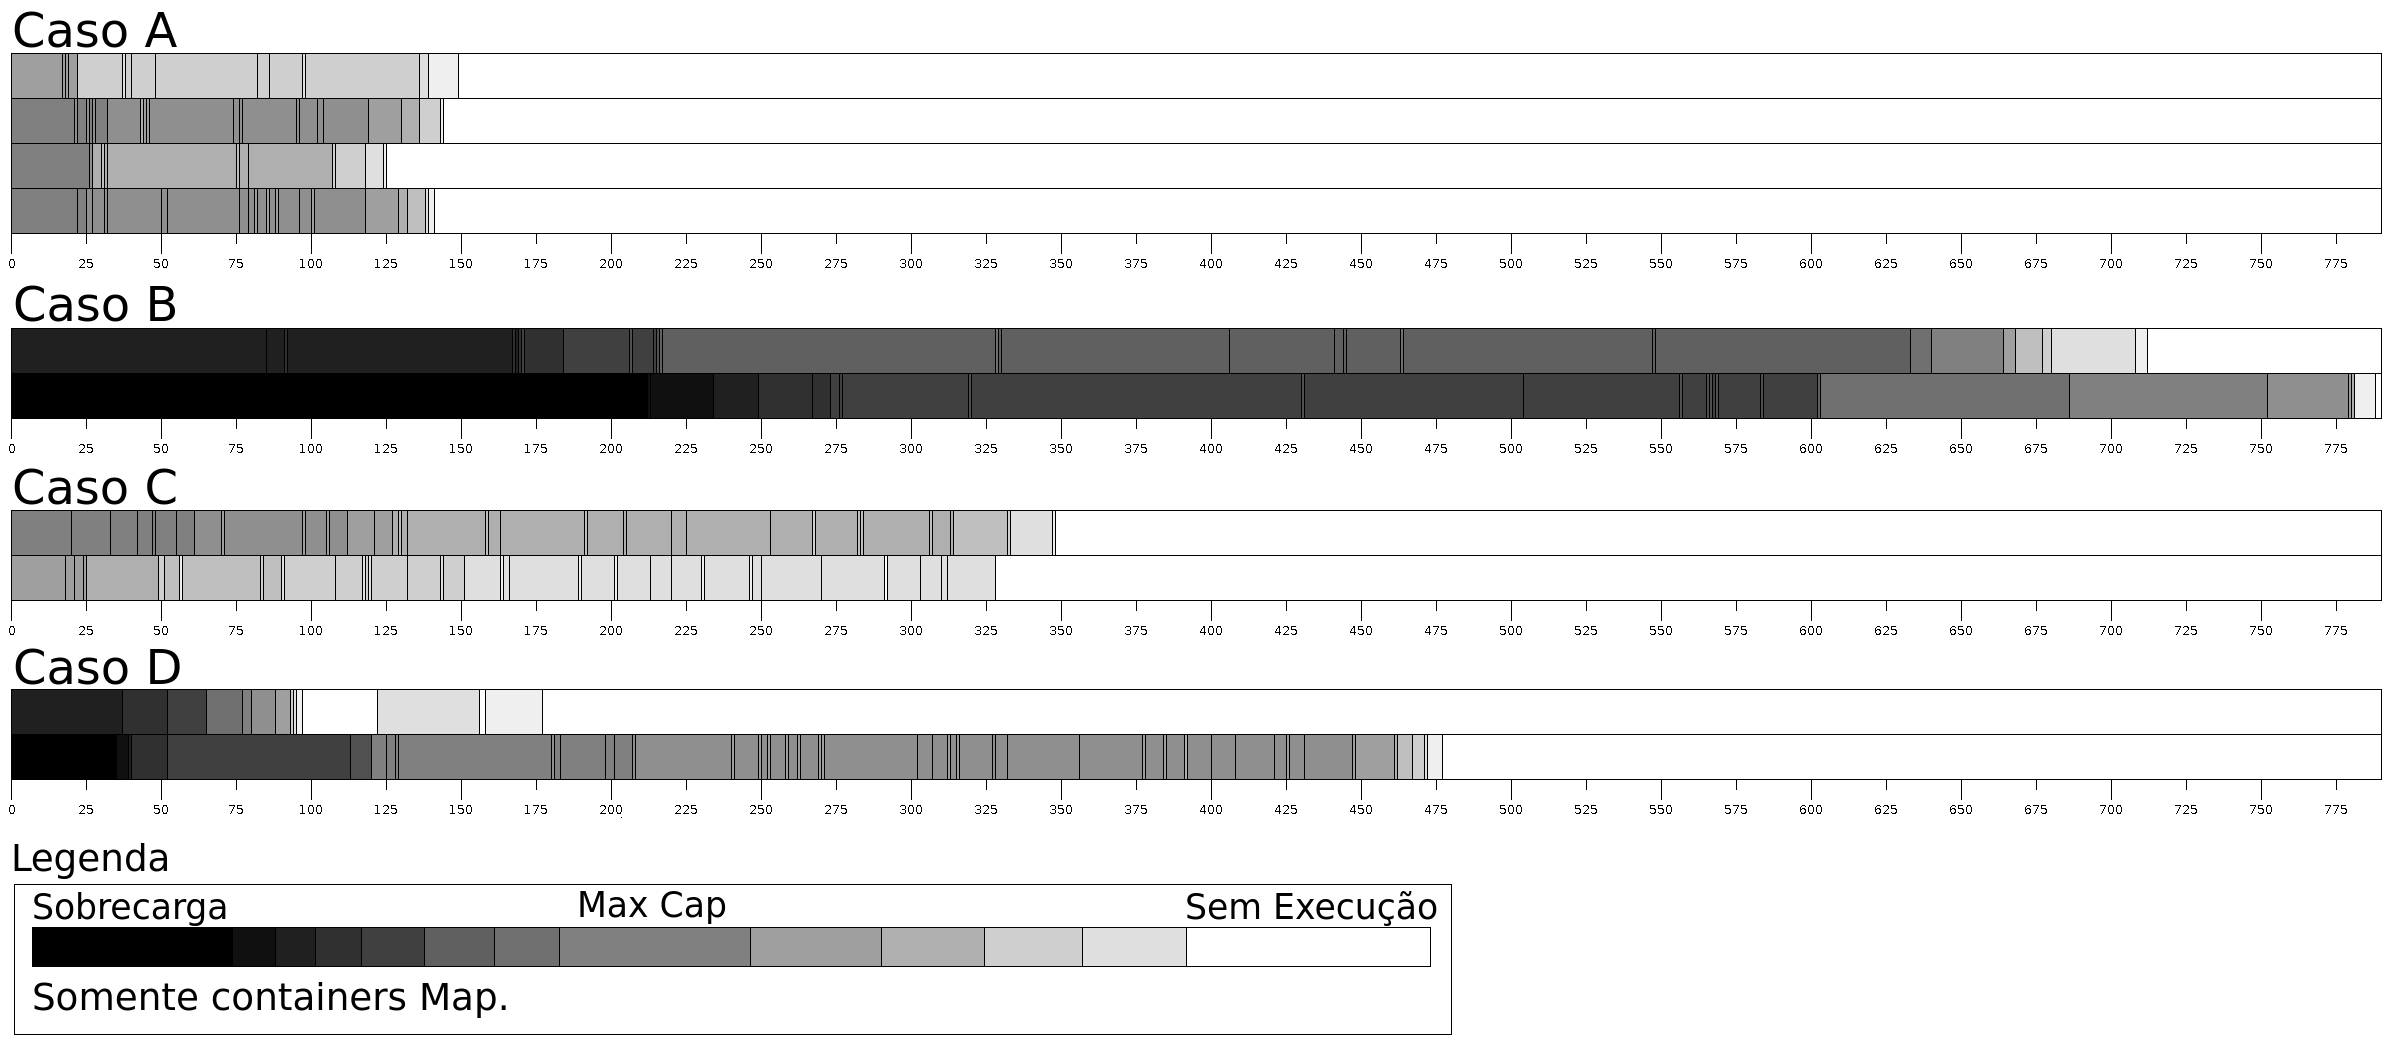
\includegraphics[width=1\textwidth]{figuras/todos.png}
	\caption{Diagrama de Gantt para os experimentos com TeraSort}
	\label{fig:exp1TS}
\end{figure}

\begin{figure}[!ht]
	\centering
	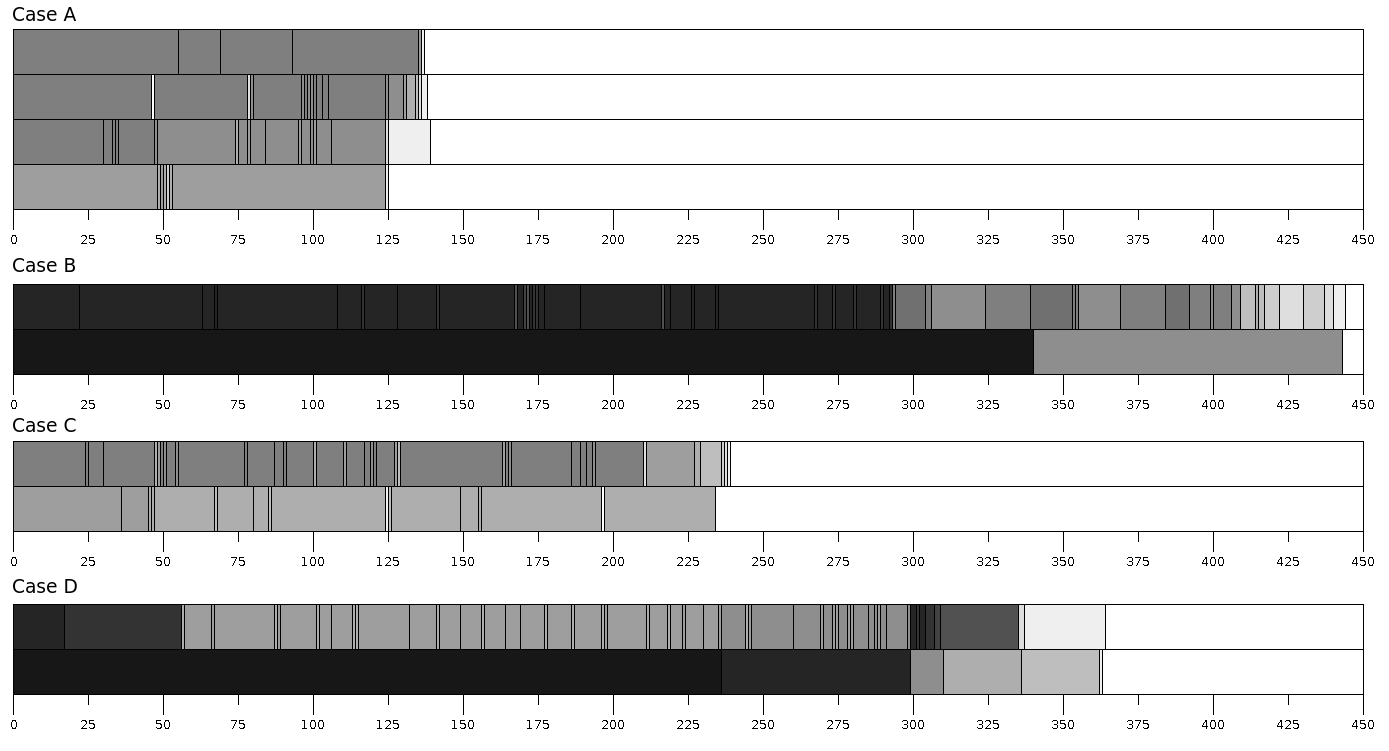
\includegraphics[width=1\textwidth]{figuras/todos-DFSIO.png}
	\caption{Diagrama de Gantt para os experimentos com TestDFSIO}
	\label{fig:exp1IO}
\end{figure}

\begin{figure}[!ht]
	\centering
	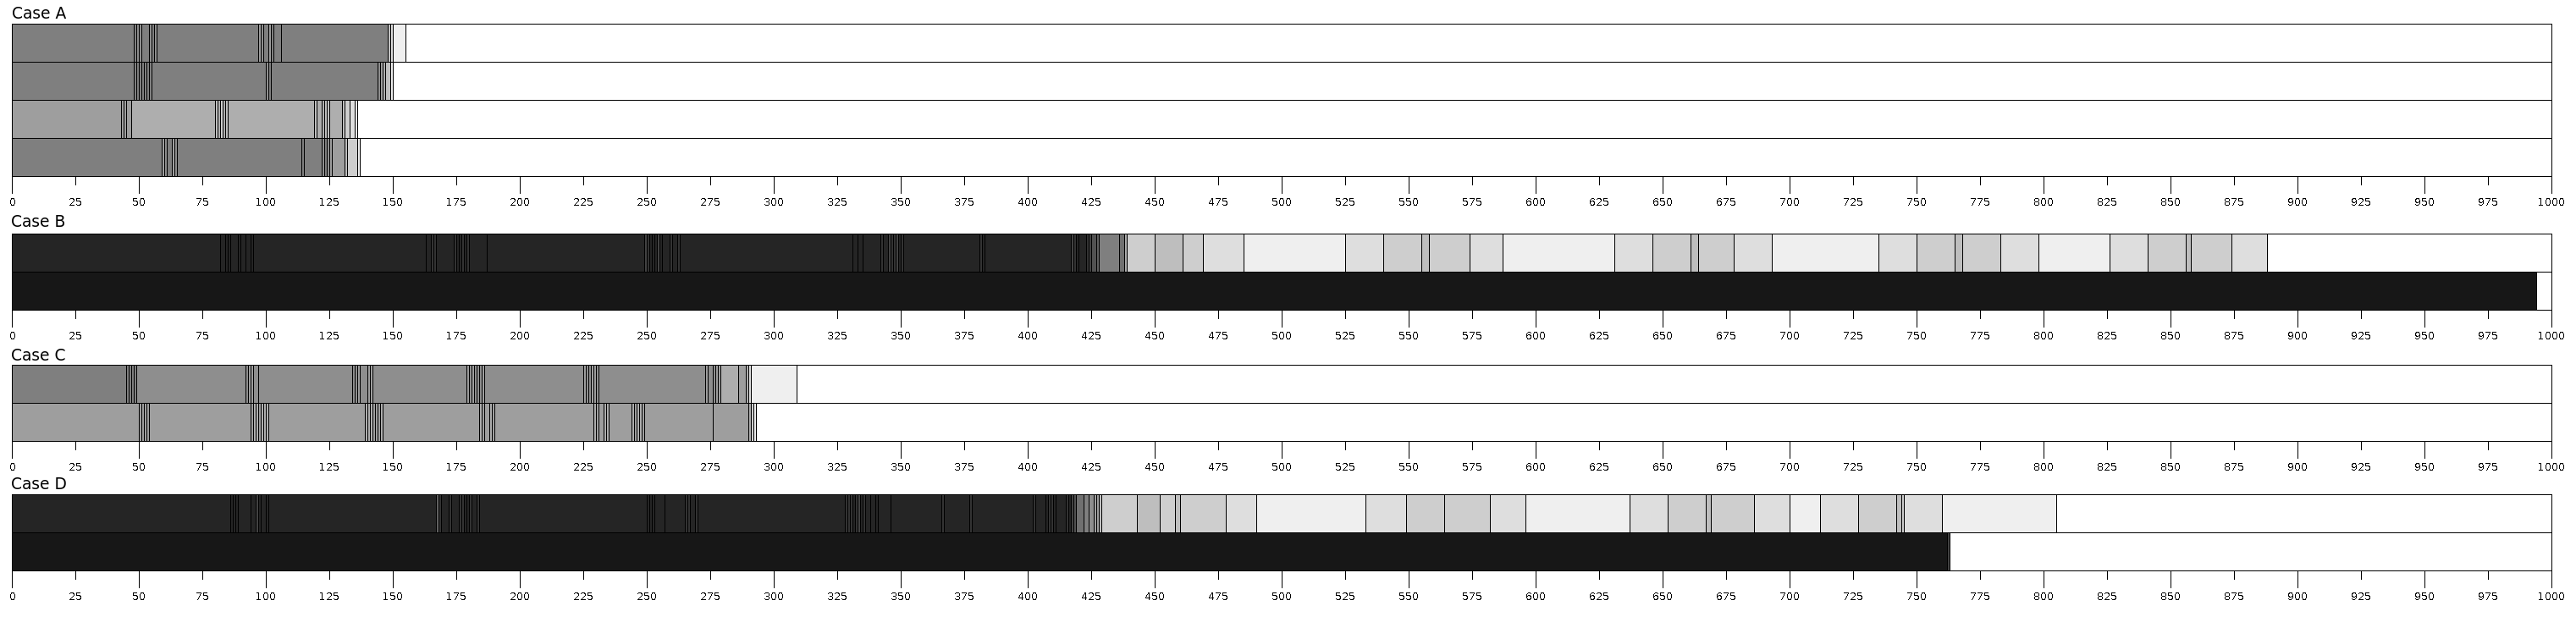
\includegraphics[width=1\textwidth]{figuras/todos-WC.png}
	\caption{Diagrama de Gantt para os experimentos com WordCount}
	\label{fig:exp1WC}
\end{figure}

\section{Experimento real}
\label{sec:expReal}
Este experimento foi realizado com objetivo de obter provas reais de que a solução apresenta melhoria no processo de escalonamento quando o Hadoop é utilizado num ambiente que existe a degradação dos recursos em virtude de compartilhamento. O experimento utiliza a solução descrita no Capítulo \ref{cap:desen}. A situação expressada com este experimento é de quando os nós do \textit{cluster} começam a ser utilizados por outros usuários antes/durante a aplicação \textit{MapReduce}.

\subsection{Configurações de Hardware e Software}
O experimento foi realizado no \textit{cluster} genepi do Grid'5000. A configuração do \textit{cluster} utilizado no experimento foi a de 1 mestre e 4 escravos, sendo que cada um destes nós possuem a seguinte configuração: 2 CPUs Intel(R) Xeon(R) E5420 2.5GHz (totalizando 8 cores por nó) e 8 GB RAM. Todos os nós do experimento possuíam o sistema operacional Ubuntu x64-12.04, com a JDK 1.8 instalada e a versão 2.6.0 do Hadoop configurada. Todas as informações foram obtidas através do sistema de \textit{logs} do Hadoop.

\subsection{Procedimentos}
Diferentemente do experimento anterior, neste experimento buscou-se o comportamento da solução em um ambiente realmente compartilhado. O \textit{cluster} possui 4 escravos e todos os escravos terão, em algum momento, seus recursos disponíveis reduzidos pela metade devido ao compartilhamento, ou seja, outra aplicação irá utilizar 4 cores e 4 GB de memória em cada nó. Para alcançar esta situação foi implementada uma aplicação em C, na qual a quantidade desejada de \textit{threads} é inicializada e cada uma delas utiliza 1 core e 1 GB de memória.

Embora aplicações de \textit{Big Data} geralmente possuem dependência de memória, outros fatores como a utilização de CPU e E/S podem influenciar no desempenho. Na busca de comprovações de que a solução apresenta ganhos quando utilizada com aplicações de diferentes características, decidiu-se pela utilização de 3 aplicações de \textit{benchmark}, cada uma com diferentes requisições de memória, CPU e E/S.

As aplicações são as seguintes:
\begin{itemize}
	\item TeraSort: o objetivo do TeraSort \citep{TeraSort2008} é ordenar um conjunto de dados o mais rápido possível. Este \textit{benchmark} de ordenação estressa tanto a memória como o CPU em virtude das comparações e armazenamento temporário;
	\item WordCount: o \textit{benchmark} WordCount é um exemplo básico de \textit{MapReduce}. Seu objetivo é contar o número de ocorrências de cada palavra de um texto. Como a utilização de memória e E/S é limitada nesta aplicação (tanto na etapa de processamento como a saída da aplicação possuem estruturas pequenas em comparação ao arquivo de entrada), o desempenho desta aplicação é determinado pelo CPU;
	\item TestDFSIO: o \textit{benchmark} TestDFSIO é um teste de leitura e escrita para o HDFS. Este \textit{benchmark} é útil para estressas o HDFS, descobrir \textit{bottlenecks} na rede, SO e configuração do Hadoop. O objetivo é prover uma mensuração de quão rápido o \textit{cluster} é em termos de E/S. Tanto a memória quanto o CPU são pouco utilizados.
\end{itemize}

Utilizou-se das aplicações implementadas no \textit{HiBench}, um conjunto de \textit{benchmarks} para \textit{clusters} Hadoop \cite{HiBench}. O tamanho de entrada utilizado para cada aplicação foi: um conjunto de dados de 15 GB para o Terasort, 90 arquivos de 250 MB para o TestDFSIO e um arquivo de 10 GB para o WordCount. 

\subsection{Casos de Teste}
Os seguintes casos de teste foram criados e configurados para os experimentos:

\textbf{Caso A:} representa uma situação sem compartilhamento, onde o usuário possui acesso à todos os recursos do \textit{cluster} em qualquer momento. Isto implica que os recursos informados ao escalonador \textbf{sempre} corresponderão aos recursos disponíveis para o Hadoop. Consideram-se recursos informados como os dados que o escalonador utiliza para realizar suas políticas de escalonamento, enquanto, recursos disponíveis são aqueles estão livres e/ou sendo utilizados pelo próprio Hadoop. Utilizando uma notação percentual, os recursos informados são de 100\% e os recursos disponíveis são de 100\% durante toda execução.

\textbf{Caso B:} representa a situação decorrente do compartilhamento dos nós do \textit{cluster} com outros usuários. Como consequência do compartilhamento, é possível que em, algum momento, ocorra uma inconsistência entre a quantidade de recursos informada e disponível. Este caso aplica o comportamento padrão do Hadoop, no qual os recursos são informados por meio de arquivos XML \textbf{somente} na inicialização do serviço e nunca são atualizados. Em notação percentual, os recursos informados são de 100\%, porém os recursos disponíveis são de 50\%.

\textbf{Caso C:} repete as especificações do Caso B, porém possui a implementação descrita no Capítulo \ref{cap:desen}. Este caso representa a situação de quando outra aplicação é lançada \textbf{antes} da ocorrência da coleta e transmissão de dados, ou seja, quando uma nova aplicação for submetida ao \textit{cluster}, este já estará com os dados atualizados. Em notação percentual, os recursos informados são de 50\% e os recursos disponíveis são de 50\%.

\textbf{Caso D:} representa uma extensão do Caso C em que a inicialização de outra aplicação ocorre \textbf{após} a coleta e transmissão dos dados e \textbf{antes} da submissão de uma aplicação, ou seja, a aplicação será lançada numa situação onde o \textit{cluster} possui a informação errada (Caso B) e terá de se adaptar à nova configuração dos recursos (Caso C) durante a execução. Em notação percentual, os recursos informados no início da aplicação são de 100\%, enquanto os recursos disponíveis são de 50\%. Após a coleta e transmissão de dados os recursos informados também passam a ser 50\%.

\subsection{Resultados e Interpretações}
The comparison of node memory from default and collector implementation can be seen in the table \ref{tab:experiments}.

\section{Experimento de escala}
Uma vez que os experimentos anteriores já responderam algumas questões importantes sobre a viabilidade da solução implementada, este experimento foi realizado com objetivo de obter provas de que a solução apresenta melhoria no processo de escalonamento mesmo quando o Hadoop é utilizado em um ambiente de grande escala com uma aplicação de grande escala. O experimento utiliza a solução descrita no Capítulo \ref{cap:desen}. A situação expressada com este experimento é de quando os nós do \textit{cluster} começam a ser utilizados por outros usuários antes/durante a aplicação \textit{MapReduce}.

\subsection{Configurações de Hardware e Software}
%TODO mudar descrição para ficar de acordo com o experimento
O experimento foi realizado no \textit{cluster} genepi do Grid'5000. A configuração do \textit{cluster} utilizado no experimento foi a de 1 mestre e 4 escravos, sendo que cada um destes nós possuem a seguinte configuração: 2 CPUs Intel(R) Xeon(R) E5420 2.5GHz (totalizando 8 cores por nó) e 8 GB RAM. Todos os nós do experimento possuíam o sistema operacional Ubuntu x64-12.04, com a JDK 1.8 instalada e a versão 2.6.0 do Hadoop configurada.

\subsection{Procedimentos}
%TODO arrumar quantidade de escravos
Neste experimento buscou-se o comportamento da solução em um ambiente realmente compartilhado e de grande escala. O \textit{cluster} possui X escravos e todos os escravos terão, em algum momento, seus recursos disponíveis reduzidos pela metade devido ao compartilhamento, ou seja, outra aplicação irá utilizar 4 cores e 4 GB de memória em cada nó. Para alcançar esta situação foi implementada uma aplicação em C, na qual a quantidade desejada de \textit{threads} é inicializada e cada uma delas utiliza 1 core e 1 GB de memória.

Embora aplicações de \textit{Big Data} geralmente possuem dependência de memória, outros fatores como a utilização de CPU e E/S podem influenciar no desempenho. Na busca de comprovações de que a solução apresenta ganhos quando utilizada com aplicações de diferentes características, decidiu-se pela utilização de 3 aplicações de \textit{benchmark}, cada uma com diferentes requisições de memória, CPU e E/S.

As aplicações são as seguintes:
\begin{itemize}
	\item TeraSort: o objetivo do TeraSort \citep{TeraSort2008} é ordenar um conjunto de dados o mais rápido possível. Este \textit{benchmark} de ordenação estressa tanto a memória como o CPU em virtude das comparações e armazenamento temporário;
	\item WordCount: o \textit{benchmark} WordCount é um exemplo básico de \textit{MapReduce}. Seu objetivo é contar o número de ocorrências de cada palavra de um texto. Como a utilização de memória e E/S é limitada nesta aplicação (tanto na etapa de processamento como a saída da aplicação possuem estruturas pequenas em comparação ao arquivo de entrada), o desempenho desta aplicação é determinado pelo CPU;
	\item TestDFSIO: o \textit{benchmark} TestDFSIO é um teste de leitura e escrita para o HDFS. Este \textit{benchmark} é útil para estressas o HDFS, descobrir \textit{bottlenecks} na rede, SO e configuração do Hadoop. O objetivo é prover uma mensuração de quão rápido o \textit{cluster} é em termos de E/S. Tanto a memória quanto o CPU são pouco utilizados.
\end{itemize}

Utilizou-se das aplicações implementadas no \textit{HiBench}, um conjunto de \textit{benchmarks} para \textit{clusters} Hadoop \cite{HiBench}. O tamanho de entrada utilizado para cada aplicação foi: um conjunto de dados de 15 GB para o Terasort, 90 arquivos de 250 MB para o TestDFSIO e um arquivo de 10 GB para o WordCount. 

\subsection{Casos de Teste}
Os seguintes casos de teste foram criados e configurados para os experimentos:

\textbf{Caso A:} representa uma situação sem compartilhamento, onde o usuário possui acesso à todos os recursos do \textit{cluster} em qualquer momento. Isto implica que os recursos informados ao escalonador \textbf{sempre} corresponderão aos recursos disponíveis para o Hadoop. Consideram-se recursos informados como os dados que o escalonador utiliza para realizar suas políticas de escalonamento, enquanto, recursos disponíveis são aqueles estão livres e/ou sendo utilizados pelo próprio Hadoop. Utilizando uma notação percentual, os recursos informados são de 100\% e os recursos disponíveis são de 100\% durante toda execução.

\textbf{Caso B:} representa a situação decorrente do compartilhamento dos nós do \textit{cluster} com outros usuários. Como consequência do compartilhamento, é possível que em, algum momento, ocorra uma inconsistência entre a quantidade de recursos informada e disponível. Este caso aplica o comportamento padrão do Hadoop, no qual os recursos são informados por meio de arquivos XML \textbf{somente} na inicialização do serviço e nunca são atualizados. Em notação percentual, os recursos informados são de 100\%, porém os recursos disponíveis são de 50\%.

\textbf{Caso C:} repete as especificações do Caso B, porém possui a implementação descrita no Capítulo \ref{cap:desen}. Este caso representa a situação de quando outra aplicação é lançada \textbf{antes} da ocorrência da coleta e transmissão de dados, ou seja, quando uma nova aplicação for submetida ao \textit{cluster}, este já estará com os dados atualizados. Em notação percentual, os recursos informados são de 50\% e os recursos disponíveis são de 50\%.

\textbf{Caso D:} representa uma extensão do Caso C em que a inicialização de outra aplicação ocorre \textbf{após} a coleta e transmissão dos dados e \textbf{antes} da submissão de uma aplicação, ou seja, a aplicação será lançada numa situação onde o \textit{cluster} possui a informação errada (Caso B) e terá de se adaptar à nova configuração dos recursos (Caso C) durante a execução. Em notação percentual, os recursos informados no início da aplicação são de 100\%, enquanto os recursos disponíveis são de 50\%. Após a coleta e transmissão de dados os recursos informados também passam a ser 50\%.

\subsection{Resultados e Interpretações}
The comparison of node memory from default and collector implementation can be seen in the table \ref{tab:experiments}.

%
%\section{Original CapacityScheduler X Context-aware CapacityScheduler}
%This experiment was performed in order to compare the container allocation pattern in the original CapacityScheduler and the context-aware CapacityScheduler. The experiment consisted in executing a TeraSort in the cluster with the original CapacityScheduler and the context-aware CapacityScheduler. This was made in order to compare how the higher resource availability and higher allocation limits impacted the scheduling.
%
%\subsection{Hardware and Software configuration}
%The experiment used the same hardware configuration from the previous one. Regarding the Hadoop configuration, there are new properties used. The properties are the minimum and maximum allocation values, which are set in properties stated on section \ref{sec:alloc}. The only difference being that one of the executions had the collector plugged.
%
%\subsection{Procedures}
%The procedure chosen as data acquisition method was the Hadoop Log System. The reason for such a choice was that Hadoop Log System is, by default, enabled in the INFO level and using the INFO level would be possible to insert small entries and extract useful information in real time. The data was acquired with the same call during the execution of services with both schedulers.
%
%The application used to test the scheduling was a TeraSort with 5GB data to sort, requesting enough containers and providing enough data to be processed in order to stress the cluster.
%
%
%\subsection{Results and interpretation}
%Before going further into the interpretation of the results, there are some characteristics of jobs that need to be reminded. If the number of reduce tasks parameter isn't set on \textit{mapred-site.XML}, the default value used is 1, making the whole reduce step forced to be executed on only one container.
%
%Another thing to note is that the first allocated container is always the ApplicationMaster, making this container not relevant in grant of resources for MapReduce tasks analysis. Thus both the ApplicationMaster and Reducer container were withdraw from the data analyzed, which was left only with the Map containers. All times are normalized related to the first Map container created.
%
%The cluster configuration achieved with the original CapacityScheduler was: 
%\begin{itemize}
%	\item Total cluster resource of 32768mb and 32cores
%	\item Minimum allocation of 1024mb and 1 core
%	\item Maximum allocation of 8192mb and 32 cores.
%	\item All Map containers were granted containers of 1024mb and 1 core, the minimum limit.
%\end{itemize}
%
%
%The cluster configuration achieved with the context-aware CapacityScheduler was: 
%\begin{itemize}
%	\item Total cluster resource of 193210mb and 96cores
%	\item Minimum allocation of 4830mb and 2 cores
%	\item Maximum allocation of 24151mb and 12 cores
%	\item All Map containers were granted containers of 4830mb and 2 cores, the minimum limit.
%\end{itemize}
%
%Although a huge difference was achieved by only comparing the resources collected and the allocation limits, the main objective of this work is to impact the scheduling performance in a Hadoop cluster. Therefore, a TeraSort execution was made and the results achieved are discussed below.
%
%The following Gantt Charts are consolidated by resources, which are the NodeManagers. This means that the tasks, in this case portrayed as containers, will be consolidated to the resources they are tied. As stated before, the containers are allocated to a certain NodeManager. The consolidation works in a way that when a separation occurs in the segment, it means that a container has either started or finished on that NodeManager. That implies that many containers will be on more than one segment, and, the numbers inside the segment indicates which containers are running at that moment.
%
%Figure \ref{fig:ganttDefault} portraits the Gantt Chart of the TeraSort with original CapacityScheduler. It is easy to notice that some containers had to wait for the completion of others in order to start processing their tasks.
%
%\begin{figure}[hbtn]
%   \renewcommand{\figurename}{Figure}
%   \centering
%   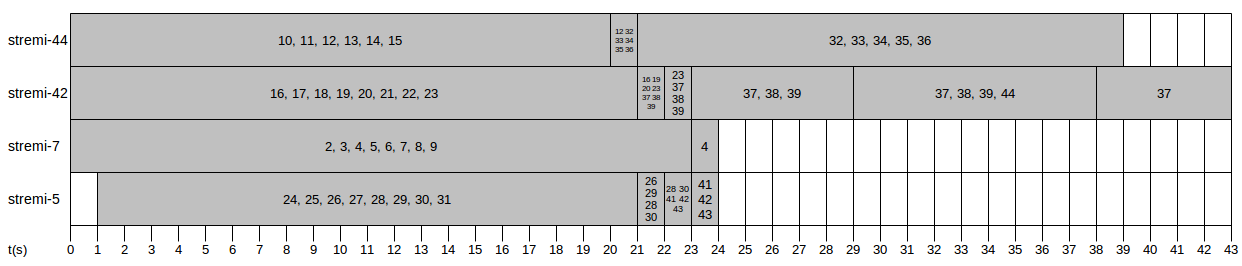
\includegraphics[width=16cm]{figuras/Figura16-GanttDefault.png}
%   \caption{Container assignment with default configuration}
%   \label{fig:ganttDefault}
%\end{figure}
%
%In order to illustrate how to interpret the Gantt charts, the node stremi-42 of figure \ref{fig:ganttDefault} will be taken as example. It starts all its containers, numbered from 16 to 23, at the 0 seconds mark, then the segment ends at the 21 seconds mark, meaning that either a container started or finished. After a quick analysis of the containers in the first and second segments, it is possible to note that containers 17, 18, 21 and 22 are not in the second segment, meaning they have finished processing their tasks. Another thing to notice is that on the second segment, containers with numbers 37, 38 and 39 appeared for the first time, meaning they were started at this time. If the analysis is extended to the segment from 22 to 23 seconds, it is possible to note that containers 16, 19 and 20 have finished processing their tasks too, and the only running containers in this node at this moment are the containers 23, 37, 38 and 39.
%
%Figure \ref{fig:ganttImproved} portraits the Gantt Chart of the TeraSort with context-aware CapacityScheduler. In this case the overall completion time was reduced, this happened due to the fact that all containers could be started right after the arrival of the request, thanks to the higher resource availability.
%
%\begin{figure}[hbtn]
%   \renewcommand{\figurename}{Figure}
%   \centering
%   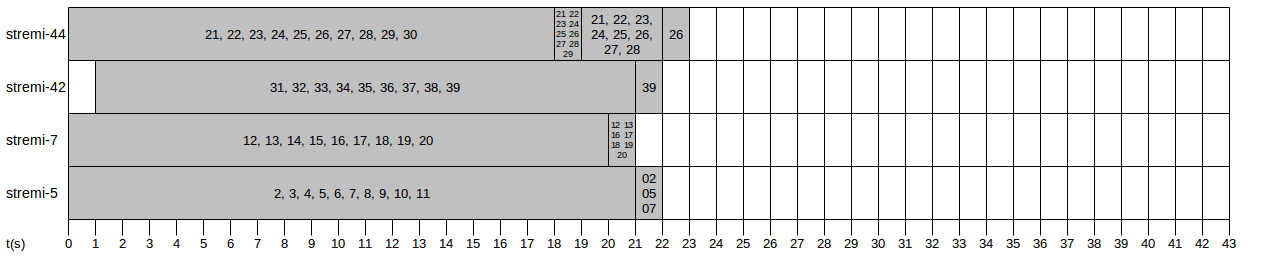
\includegraphics[width=15cm]{figuras/Figura17-GanttImproved.png}
%   \caption{Container assignment with the improved configuration}
%   \label{fig:ganttImproved}
%\end{figure}
%
%After an analysis and comparison of both charts, it is possible to notice that the default chart has containers 41-43 started on node stremi-5 and container 44 started on node stremi-42, while the context-aware chart has only the standard containers, which are numbered 2-39. This happens because these extra containers are, in reality, speculative tasks launched because other tasks were taking to long to finish. Without a better information acquisition it is hard to determine the match of original and speculative containers, but it is possible to infer which containers would make possible candidates, leaving containers 2-9, 23, 28 and 30 as possible staggers, responsible for the launching of speculative containers 41-43. Because of the same reasons, it is only possible to infer that container 44 was launched because the most likely stagger was one container in the 32-36 range.
%
%By analysing the container numberings it is possible to notice how the scheduler decides which node is going to be used. The containers launched on a given node follow a logic numbering, meaning that the resources of that container are used until exhaustion before the scheduler starts launching containers on another node. 

%\section{Heterogeneity simulation}
%This experiment was performed in order to simulate a heterogeneous environment and test how well would the context-aware would adapt. The experiment consisted in executing a TeraSort in the cluster with the simulated heterogeneous environment using context-aware CapacityScheduler. 
%
%\subsection{Hardware and Software configuration}
%The experiment used the same hardware configuration from the previous experiments. Regarding the Hadoop configuration, there are no changes. The only difference is that the nodes are purposely given false capacities when being added to the RM. Using this false values, a heterogeneous cluster will be simulated.
%
%\subsection{Procedures}
%The procedure chosen as data acquisition method was the Hadoop Log System. The reason for such a choice was that Hadoop Log System is, by default, enabled in the INFO level and using the INFO level would be possible to insert small entries and extract useful information in real time. The data was acquired with the same call during the execution of services with both schedulers.
%
%The application used to test the scheduling was a TeraSort with 5GB data to sort, requesting enough containers and providing enough data to be processed in order to stress the cluster.
%
%\subsection{Results and interpretation}
%As this experiment is a replication of the last one plus the simulated heterogeneity, the same principles applies regarding the container analysis. 
%
%It is important to firstly know the configuration of the simulated heterogeneity. The cluster had the following simulated configuration:
%
%\begin{itemize}
%	\item stremi-17: 28981 MB of memory and 14 cores.
%	\item stremi-22: 34715 MB of memory and 18 cores.
%	\item stremi-33: 46287 MB of memory and 24 cores.
%	\item stremi-35: 24151 MB of memory and 12 cores.
%	\item Total Cluster Resources: 134134 MB of memory and 68 cores.
%	\item Minimum Allocation: 3353 MB of memory and 1 core.
%\end{itemize}
%
%Figure \ref{fig:ganttSimulation} portraits the Gantt Chart of the TeraSort execution within the simulated heterogeneous environment, also using context-aware CapacityScheduler. Compared to the default case, the heterogeneous environment execution shows an improvement, but due to the lower cluster capacity, it is a slightly worse than the context-aware CapacityScheduler executing on a homogeneous environment.
%
%\begin{figure}[hbtn]
%   \renewcommand{\figurename}{Figure}
%   \centering
%   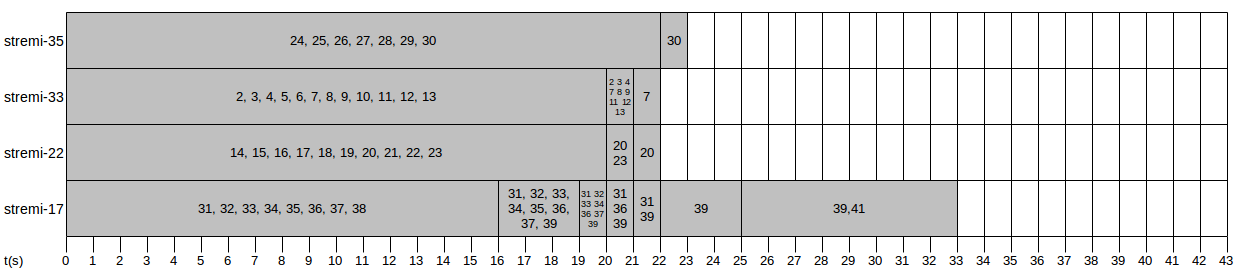
\includegraphics[width=15cm]{figuras/Figura21-GanttSimulation.png}
%   \caption{Container assignment with the simulated heterogeneous environment}
%   \label{fig:ganttSimulation}
%\end{figure}
%
%It is possible to note that the containers started the assignment with the node stremi-33, which is the node with the most capacity in the cluster and also was the first to be added in the node list. As in the other experiments, the scheduler launches containers on a node until its resources are all reserved, then mode to the next node on the list.
%
%On this experiment a speculative task was launched. Contrary to the other experiments, its easy to infer which was the original stagger task, since there was only one container active at the moment that the container 41 was launched. It is also possible to note that the scheduler didn't change nodes to launch the speculative, that happens because the node had spare capacity when the request for the speculative arrived.
%
%This experiment shows that it is possible to use this context-aware in a heterogeneous environment, the allocations were adapted to a slightly smaller cluster if compared to the real environment. As a future work, it is possible to set the allocation limits in function not only of total cluster resources but also of each individual node resource capacity.